\documentclass[english]{article}

\bibliographystyle{unsrt}

% Section
\newcommand{\secref}[1]{Subsection~\ref{sec.#1}}
\newcommand{\seclabel}[1]{\label{sec.#1}}

% Appendix
\newcommand{\appref}[1]{Appendix~\ref{app.#1}}
\newcommand{\applabel}[1]{\label{app.#1}}

% Table
\newcommand{\tabnum}[1]{\ref{tab.#1}}
\newcommand{\tabref}[1]{Table~\tabnum{#1}}
\newcommand{\tablabel}[1]{\label{tab.#1}}

% Equation
\newcommand{\eqnref}[1]{Equation~\ref{Equations.#1}}
\newcommand{\eqnlabel}[1]{\label{Equations.#1}}

% Figure
\newcommand{\figref}[1]{Figure~\ref{Figures.#1}}
\newcommand{\figlabel}[1]{\label{Figures.#1}}

\newcommand{\easyfig}[4]{
\begin{figure}
\includegraphics[#2]{#1}
\caption{ \figlabel{#3} #4}
\end{figure}}

\newcommand{\dotfig}[4]{
\begin{figure}
\input{#1.tex}
\includegraphics[#2]{#1.ps}
\caption{ \figlabel{#3} #4}
\end{figure}}

\newcommand{\pngfig}[2]{\easyfig{#1.png}{}{#1}{#2}}
\newcommand{\pdffig}[2]{\easyfig{#1-fig.pdf}{}{#1}{#2}}

\newcommand{\widepngfig}[2]{\easyfig{#1.png}{width=\textwidth}{#1}{#2}}
\newcommand{\tallpngfig}[2]{\easyfig{#1.png}{height=.8\textheight}{#1}{#2}}
\newcommand{\widepdffig}[2]{\easyfig{#1-fig.pdf}{width=\textwidth}{#1}{#2}}
\newcommand{\tallpdffig}[2]{\easyfig{#1-fig.pdf}{height=.8\textheight}{#1}{#2}}

\newcommand{\sidewayspngfig}[2]{
\begin{sidewaysfigure}
\includegraphics[width=\textwidth]{#1.png}
\caption{\figlabel{#1} #2}
\end{sidewaysfigure}
}

% ToDo
\newcommand{\needfig}[1]{{\bf Need figure: } #1 }
\newcommand{\needfigref}[1]{Figure~??? [#1] }

\newcommand{\needcite}[1]{[CITE #1]}
\newcommand{\todo}[1]{[TODO: #1]}

% Packages

\usepackage[boxed,noend]{algorithm2e}
\usepackage{graphicx}
\usepackage{psfrag}
\usepackage{url}
\usepackage{amsmath}
\usepackage{amssymb}
\usepackage{color} 
\usepackage{ifthen}
\usepackage{rotating}
\newcommand{\hl}[1]{#1}

\newcommand\semiring{K}
\newcommand\srset{\mathbb{K}}
\newcommand\srplus{\oplus}
\newcommand\srtimes{\otimes}
\newcommand\srplusid{\underline{0}}
\newcommand\srtimesid{\underline{1}}
\newcommand\srsum{\bigoplus}
\newcommand\srprod{\bigotimes}

\newcommand\inalph{\Sigma}
\newcommand\outalph{\Omega}
\newcommand\states{Q}
\newcommand\transitions{E}
\newcommand\initstate{i}
\newcommand\finalstate{f}
\newcommand\emptystring{\epsilon}
\newcommand\maybe[1]{#1 \cup \{ \emptystring \}}

\newcommand\state{q}
\newcommand\trans{t}
\newcommand\src{p}
\newcommand\dest{q}
\newcommand\lab{\ell}
\newcommand\inlab{\lab_i}
\newcommand\outlab{\lab_o}
\newcommand\weight{\mathbb{W}}

\newcommand\somealph{\Gamma}
\newcommand\someseq{\gamma}
\newcommand\midlab{\lab_m}

\newcommand\transcomp{\circ}
\newcommand\transconcat{+}

\newcommand\inseq{\sigma}
\newcommand\outseq{\omega}

\newcommand\kleene[1]{{#1}^{\ast}}
\newcommand\inseqs{\kleene{\inalph}}
\newcommand\outseqs{\kleene{\outalph}}
\newcommand\someseqs{\kleene{\somealph}}

\newcommand\tfunc[1]{\mathbb{#1}}

\newcommand\bigo{{\cal O}}

\newcommand\seqof[1]{\bar{#1}}
\newcommand\sympast{v}
\newcommand\symnext{w}
\newcommand\seqpast{\seqof{\sympast}}
\newcommand\seqnext{\seqof{\symnext}}

\newcommand\nucalph{\somealph_{\mbox{\tiny DNA}}}
\newcommand\sym{x}
\newcommand\comp[1]{\tilde{#1}}
\newcommand\revcomp[1]{\comp{#1}}
\newcommand\ntrans[1]{\hat{#1}}
\newcommand\seqlen[1]{|#1|}
\newcommand\otherseq{\lambda}

\newcommand\kmerlen{{\cal K}}
\newcommand\invreplen{L_{\mbox{\tiny invrep}}}

\newcommand\graph{{\cal G}}
\newcommand\vertices{{\cal V}}
\newcommand\edges{{\cal E}}

\newcommand\debruijngraph{\graph_b}
\newcommand\debruijnvertices{\vertices_b}
\newcommand\debruijnedges{\edges_b}

\newcommand\norepgraph{\graph_r}
\newcommand\norepvertices{\vertices_r}
\newcommand\norepedges{\edges_r}

\newcommand\controlgraph{\graph_c}
\newcommand\controlbridges[1]{\vertices_c(#1)}

\newcommand\prequels{{\cal S}}
\newcommand\stepsto{{\cal L}}

\newcommand\ncontrols{N_c}
\newcommand\controlset{{\cal M}}
\newcommand\controlword{M}

\newcommand\initword{\controlword_i}
\newcommand\finalword{\controlword_f}

\newcommand\initvertex[1]{u^{(#1)}_i}
\newcommand\finalvertex[1]{v^{(#1)}_f}

\newcommand\controlmachine{T_c}

\newcommand\bit[1]{#1_2}
\newcommand\trit[1]{#1_3}
\newcommand\quat[1]{#1_4}
\newcommand\controlsym[1]{{#1}_M}
\newcommand\flushsym{F}

\newcommand\figtrans[2]{T_{\ref{Figures.#1}#2}}
\newcommand\solefigtrans[1]{T_{\ref{Figures.#1}}}

\newcommand\transsingle[2]{T_{#1 \to #2}}
\newcommand\transid[1]{\transsingle{#1}{#1}}
\newcommand\transerase[1]{\transsingle{#1}{\epsilon}}

\newcommand\rbit[1]{#1_{2R}}

\newcommand\hammingthreeone{\figtrans{HammingTransducer}{a}}
\newcommand\hammingsevenfour{\figtrans{HammingTransducer}{b}}

\newcommand\transbintoquat{\figtrans{NaiveDNATransducer}{a}}
\newcommand\transquattodna{\figtrans{NaiveDNATransducer}{b}}
\newcommand\transbintodna{\figtrans{NaiveDNATransducer}{c}}

\newcommand\transdivthree{\figtrans{DivisionByThree}{a}}
\newcommand\transternzeroid{\figtrans{DivisionByThree}{b}}
\newcommand\transternsymid{\figtrans{DivisionByThree}{c}}
\newcommand\transternseqid{\figtrans{DivisionByThree}{d}}
\newcommand\transerasezerobits{\figtrans{DivisionByThree}{e}}
\newcommand\transechodivthree{\figtrans{DivisionByThree}{f}}

\newcommand\transmixed{\figtrans{Converter}{a}}
\newcommand\transflush{\figtrans{Converter}{b}}

\newcommand\transechodivtwo{\figtrans{EvenDivision}{a}}
\newcommand\transechodivfour{\figtrans{EvenDivision}{b}}
\newcommand\transechodivmixed{T_{2 \to 234}}

\newcommand\transpartial{\figtrans{PartialObservation}{c}}

\newcommand\nuc[1]{\mbox{#1}}
\newcommand\nuca{\nuc{A}}
\newcommand\nucc{\nuc{C}}
\newcommand\nucg{\nuc{G}}
\newcommand\nuct{\nuc{T}}

\newcommand\contextlen{L}
\newcommand\seqsyms[2]{\sym_{#1} \ldots \sym_{#2}}
\newcommand\seqpastsyms[2]{\sympast_{#1} \ldots \sympast_{#2}}
\newcommand\seqnextsyms[2]{\symnext_{#1} \ldots \symnext_{#2}}
\newcommand\outsym{y}

\newcommand\param[1]{\mathbb{P}_{#1}}

\newcommand\pnogap{\param{n}}
\newcommand\pdelopen{\param{d}}
\newcommand\ptandup{\param{t}}
\newcommand\pfwddup{\param{f}}
\newcommand\prevdup{\param{r}}

\newcommand\pdelext{\param{x}}
\newcommand\pdelend{\param{e}}

\newcommand\pmatch{\param{m}}
\newcommand\ptransition{\param{i}}
\newcommand\ptransversion{\param{v}}

\newcommand\submat{\param{s}}
\newcommand\lendist{\param{l}}

\newcommand\psub{\submat(\sym,\outsym)}
\newcommand\psubnext[1]{\submat(\symnext_{#1},\outsym)}
\newcommand\psubpast[1]{\submat(\sympast_{#1},\outsym)}
\newcommand\psubcomppast[1]{\submat(\sympast_{#1},\comp{\outsym})}
\newcommand\psubcompnext[1]{\submat(\symnext_{#1},\comp{\outsym})}

\newcommand\plen[1]{\lendist(#1)}

\newcommand\pcont{\pnogap^\ast}

\newcommand\block{\alpha}
\newcommand\srcblock{\block}
\newcommand\destblock{\beta}

\newcommand\blockstate[2]{{#1}_{#2}}
\newcommand\lenstate[3]{\blockstate{#1}{#2}^{(#3)}}

\newcommand\symstate[1]{\blockstate{S}{#1}}
\newcommand\delstate[1]{\blockstate{D}{#1}}
\newcommand\tanstate[2]{\lenstate{T}{#1}{#2}}
\newcommand\fwdstate[2]{\lenstate{F}{#1}{#2}}
\newcommand\revstate[2]{\lenstate{R}{#1}{#2}}

\begin{document}

\newcommand\authorstring{
Ian Holmes$^{1,\ast}$ \\
\textbf{1} Department of Bioengineering, University of California, Berkeley, CA, USA \\
$\ast$ E-mail: ihh@berkeley.edu
}

\newcommand\titlestring{Modular non-repeating codes for DNA storage}
\newcommand\shorttitlestring{Modular codes for DNA}
\markboth{\shorttitlestring}{\shorttitlestring}
\begin{flushleft}
{\Large \textbf{\titlestring} } \\
\authorstring
\end{flushleft}

%\section{Abstract}
% Algorithms, implementations, empirical results

%\paragraph{Keywords:}
%\tableofcontents

\section{Introduction}

DNA can store petabytes of information per gram \cite{GoldmanEtAl2013} and can last intact for tens of thousands of years \cite{GreenEtAl2010}.
This makes it an appealing prospect for long-term archival storage.
However, DNA synthesis, sequencing, and replication are prone to errors, which may limit its potential as a storage medium \cite{ChurchEtAl2012}.
These errors can be controlled by applying the tools of information theory,
treating DNA storage as a noisy channel coding problem.

Recently, several coding schemes for DNA storage have been proposed
that address the interrelated issues of error avoidance, error correction and redundancy
\cite{GoldmanEtAl2013,MilenkovicEtAl2005,YazdiEtAl2015,GuptaEtAl2015,MilenkovicEtAl2014,MilenkovicEtAl2015,GabrysEtAl2015,MilenkovicEtAl2016,BornholtEtAl2016}.
Goldman {\em et al} \cite{GoldmanEtAl2013} synthesized DNA using a trinary (radix-3) code that avoids repeated nucleotides
(somewhat similarly to a technique known as ``run-length limitation'' in coding theory),
synthesizing to fourfold redundancy for additional error correction.
Gupta {\em et al} introduced a trinary Golay code for error correction \cite{GuptaEtAl2015}.
Strauss {\em et al} improved on Goldman {\em et al}'s redundancy using an exclusive-or method.
Milenkovic {\em et al} have published extensively in this area,
considering the avoidance of DNA structure in codes \cite{MilenkovicEtAl2005},
proposing several codes and analyzing their combinatoric properties \cite{MilenkovicEtAl2014,MilenkovicEtAl2015,GabrysEtAl2015,MilenkovicEtAl2016}
and devising a random-access rewritable filesystem \cite{YazdiEtAl2015}.
A parallel body of work describes error-correcting codes for noisy channels that are subject to
substitutions, insertions and deletions \cite{DaveyMackay2000,DaveyMackay2001}.

Here we describe a modular strategy for constructing error-tolerant DNA codes.
As noted above, much recent work has used Goldman {\em et al}'s trinary code as a starting point.
The trinary code arises from avoidance of dinucleotide repeats, which leaves 3 available possibilities at each position, hence the radix of 3.
The rationale for this system advanced by Goldman {\em et al} is that it guards against the most common class of errors in DNA resequencing which occur at homopolymer runs.
However, there are hidden assumptions in this reasoning, specifically that it is worth making synthesis a bit more expensive in order to improve sequencing.
This may indeed be the case, but (for the moment at least) synthesis is vastly more expensive than sequencing,
so we might want to pack in more information---and yet still (perhaps) avoid certain motifs in the synthesized DNA,
such as restriction enzyme sites, or barcodes, or other sequences that have special significance in our DNA filesystem.
Alternatively, assuming a world where synthesis is cheap and yet sequencing and bioinformatics have not solved the problem of decoding homopolymer runs
(an assumption which might motivate the trinary code),
it may then be desirable to avoid other sources of error, such as repeated dinucleotides, trinucleotides or longer repeats.
Avoiding these sequences does not reduce the information content of DNA much, but they are comparable to homopolymer runs in their error rate.
We may also wish to introduce error-correcting codes such as Hamming codes \cite{Mackay2003}, Golay codes \cite{GuptaEtAl2015},
turbo codes \cite{FreyMackay98,MurphyEtAl1999}, or Gallager codes \cite{Mackay1997}.

In short, different applications may require different codes.
As noted above, several researchers have presented solutions to some of these problems.
Here, we combine some of the ideas using a modular strategy for code design.
Codes can be designed using this method to meet flexible needs
including error-avoidance, error-correction, and demarcation of metadata.

The core idea of our approach is to convert raw binary data (possibly interleaved with filesystem metadata) into a mixed-radix sequence
wherein successive digits may be binary (radix-2), trinary (radix-3) or quaternary (radix-4).
The radix at any given position is effectively specified by the number of nucleotides available for coding at that position
(which may vary due to avoidance of repeats or reserved motifs).
The mixed-radix sequence can then be efficiently converted to a DNA sequence.
Error-correcting codes (for example, Hamming codes that introduce parity bits)
can be applied upstream of the conversion from binary to mixed-radix,
while the readout process (errors from which may reintroduce repeats and prohibited motifs)
can be integrated into the decoding model as a step that follows the conversion from mixed-radix to DNA.

Our strategy uses several techniques familiar in bioinformatics and signal processing:
De Bruijn graphs, finite-state transducers, and arithmetic coding.
Transducers \cite{MohriPereiraRiley2000,WikipediaTransducers} are used as automata-theoretic models of sequence transformation
to represent in a uniform way the various steps of error-correction (e.g. via introduction of parity bits),
adix conversion, repeat-avoidant nucleotide encoding, and a statistical error model.
Standard algorithms for transducer combination (e.g. transducer composition)
and decoding (Viterbi) can then be used.
Transducers have been previously used in bioinformatics for
protein classification \cite{EskinEtAl2000},
phylogenetic indel models \cite{PatenEtAl2008,WestessonEtAlArxiv2012,WestessonEtAl2012},
and cancer informatics \cite{SchwarzEtAl2014}
To construct the non-repeating transducer
we make use De Bruijn graphs
and their relationship to automata with limited context (``order-$N$ Markov models'').
Transducers are widely used for genome assembly \cite{DeBruijn1946,PevznerEtAl2001,ZerbinoBirney2008,IqbalEtAl2012},
while order-$N$ Markov models are often employed for gene-finding \cite{BurgeKarlin1997,SalzbergEtAl1999}.
To convert a binary sequence into a mixed-radix sequence we borrow concepts from the arithmetic coding algorithm \cite{Rissanen1976,Mackay2003}
and from data compression in generally; similar concepts have been used to design compression schemes for high-volume
bioinformatics datasets \cite{HsiYangEtAl2011}.

\section{Methods}

\secref{Preliminaries} reviews preliminary concepts such as operations on weighted finite-state transducers,
De Bruijn graphs, and patterns in DNA.
\secref{DeBruijnTransducer} describes the repeat-avoiding transducer that accepts a mixed-radix sequence on its input
and generates a DNA sequence without homopolymers, short microsatellites or other local repeats.
\secref{Arithmetic} develops a transducer motivated by the arithmetic compression algorithm
that converts a binary input sequence into a mixed-radix sequence suitable for subsequent encoding as DNA.
\secref{ErrorModel} describes an error-model transducer that mutates and deletes bases and reintroduces repeats.
\secref{ErrorCorrection} shows how all these transducers can be combined, together with transducers that implement error-correcting codes.

\subsection{Preliminary concepts}
\seclabel{Preliminaries}

\subsubsection{Weighted finite-state transducers}

Following \cite{MohriPereiraRiley2000}:
Assume a general semiring
$\semiring=(\srset,\srplus,\srtimes,\srplusid,\srtimesid)$
which for our purposes is typically the probability semiring
$(\Re,+,\times,0,1)$
or the tropical semiring
$(\Re_{+} \cup {\infty},\min,+,\infty,0)$.

A weighted finite-state transducer is defined as a tuple
$\trt = (\inalph,\outalph,\states,\transitions,\initstate,\finalstate)$
consisting of an input alphabet $\inalph$,
an output alphabet $\outalph$ (both alphabets being finite sets),
a finite set of states $\states$,
a finite set of transitions
$\transitions \subseteq \states \times (\maybe{\inalph}) \times (\maybe{\outalph}) \times \srset \times \states$,
an initial state $\initstate \in \states$
and a final state $\finalstate \in \states$.

The transducer $\trt$ can be thought of as an edge-labelled directed graph
where each state is a vertex
and each transition
$\trans = (\src[\trans],\inlab[\trans],\outlab[\trans],\weight[\trans],\dest[\trans]) \in \transitions$
is an edge from state $\src[\trans]$ to state $\dest[\trans]$
with input label $\inlab[\trans]$,
output label $\outlab[\trans]$
and weight $\weight[\trans]$.

A path in $\trt$ is a series of transitions that form a path in this graph.
The input sequence and output sequence for a path are the concatenation of (respectively)
the input and output labels of the transitions in the path.
The path weight is the $\srtimes$-product of the transition weights.
A successful path is one that starts in $\initstate$ and ends in $\finalstate$.
The transduction weight for a given input sequence $\inseq \in \inseqs$
and output sequence $\outseq \in \outseqs$
is the $\srplus$-sum of all successful paths
having $\inseq$ as the input sequence
and $\outseq$ as the output sequence.
Thus $\trt$ provides a mapping
$\tfunc{T}:(\kleene{\inalph} \times \kleene{\outalph}) \to \srset$
from sequence-pairs to weights.
We call this mapping $\tfunc{T}$ the transducer function.
For a given pair of sequences $(\inseq,\outseq)$
and a semiring wherein $\srplus$ and $\srtimes$ are amortized-constant resource operations,
it can be evaluated in time $\bigo(|\inseq| \cdot |\outseq| \cdot |\transitions|)$
and memory $\bigo(|\inseq| \cdot |\outseq| \cdot |\states|)$
by dynamic programming,
analogously to the Forward algorithm in the probabilistic semiring
or the Viterbi algorithm in the tropical semiring
\cite{Durbin98}.

A state $\state \in \states$ has past input context $\seqpast$ if every path from $\initstate$ to $\state$ has an input sequence with suffix $\seqpast$,
and future input context $\seqnext$ if every path from $\state$ to $\finalstate$ has an input sequence with prefix $\seqnext$.
The past output context and future output context of a state are defined similarly.

A ``waiting state'' is a state that has no outgoing transitions with empty input labels.
A ``waiting machine'' is a transducer where all the transitions with nonempty input labels
originate from waiting states.
Any transducer $\trt$ with a transducer function $\tfunc{T}$
can be transformed into an equivalent waiting machine
that has the same transducer function $\tfunc{T}$ and
at most $2|\states|$ states and $|\states|+|\transitions|$ transitions
\cite{WestessonEtAlArxiv2012}.

\subsubsection{Transducer composition}
\seclabel{TransducerComposition}

Given transducers
 $\trr = (\inalph, \somealph, \tpr{\states}, \tpr{\transitions}, \tpr{\initstate}, \tpr{\finalstate})$ and
 $\trs = (\somealph, \outalph, \tps{\states}, \tps{\transitions}, \tps{\initstate}, \tps{\finalstate})$
where $\trr$'s output alphabet is the same as $\trs$'s input alphabet,
we can readily find a composite transducer
 $\trt = \trr \transcomp \trs = (\inalph, \outalph, \tpt{\states}, \tpt{\transitions}, \tpt{\initstate}, \tpt{\finalstate})$
such that, if $\tfunc{R}$, $\tfunc{S}$ and $\tfunc{T}$ are the corresponding transducer functions,
then
\[
\forall \inseq \in \inseqs, \outseq \in \outseqs:
\quad
\tfunc{T}(\inseq,\outseq) = \srsum_{\someseq \in \someseqs} \tfunc{R}(\inseq,\someseq) \tfunc{S}(\someseq,\outseq)
\]
that is, $\trt$ models the feeding of $\trr$'s output into $\trs$'s input
(and this intermediate sequence is then summed out---i.e. marginalized, if we are in the probabilistic semiring).

Loosely speaking, we can construct $\trt$ using the following recipe:
\begin{itemize}
\item Each $\trt$-state corresponds to a pair of $\trr$- and $\trs$-states,
so $\tpt{\state} = (\tpr{\state}, \tps{\state})$
and $\tpt{\states} \subseteq \tpr{\states} \times \tps{\states}$.
\item The initial $\trt$-state $\tpt{\initstate}=(\tpr{\initstate},\tps{\initstate})$ pairs the initial states of $\trr$ and $\trs$.
\item The final $\trt$-state $\tpt{\finalstate}=(\tpr{\finalstate},\tps{\finalstate})$ pairs the final states of $\trr$ and $\trs$.
\item $\trt$-transitions
$\tpt{\trans} = ((\tpr{\src},\tps{\src}),\inlab,\outlab,\tpt{\weight},(\tpr{\dest},\tps{\dest}))$
represent (summaries of sets of) synchronized pairs of $\trr$-transitions
$\tpr{\trans} = (\tpr{\src},\inlab,\midlab,\tpr{\weight},\tpr{\dest})$
and $\trs$-transitions
$\tps{\trans} = (\tps{\src},\midlab,\outlab,\tps{\weight},\tps{\dest})$
which share the same intermediate label $\midlab$.
The composite transition weight $\tpt{\weight}$ is the product $\tpr{\weight} \srtimes \tps{\weight}$,
or the sum over such products if there are multiple transition-pairs $(\tpr{\trans},\tps{\trans})$
consistent with a given $\tpt{\trans}$
(which, in the probabilistic semiring, is equivalent to marginalizing out $\midlab$).
\item Some additional manipulation is required to synchronize
transitions involving empty input labels (``insertions''),
empty output labels (``deletions''),
or both (``null transitions'').
For example, we can require that $\trs$ is a waiting machine,
and that $\trr$ can only change state when $\trs$ is in a waiting state \cite{WestessonEtAlArxiv2012}.
\end{itemize}

This algorithm can be made precise enough to automate;
more detailed workings are given elsewhere \cite{PereiraRiley1996,MohriPereiraRiley2000,Holmes2003,Holmes2007,WestessonEtAlArxiv2012,WestessonEtAl2012}.
The transducers yielded by a fully automated implementation can typically be aggressively optimized by hand
to minimize the number of transitions and/or states,
and hence,
the time and/or memory complexity of dynamic programming algorithms.

\subsubsection{Transducer concatenation}

Another operation on transducers that is useful in constructing DNA codes
is concatenation.
Suppose
 $\tra = (\inalph, \outalph, \tpa{\states}, \tpa{\transitions}, \tpa{\initstate}, \tpa{\finalstate})$ and
 $\trb = (\inalph, \outalph, \tpb{\states}, \tpb{\transitions}, \tpb{\initstate}, \tpb{\finalstate})$
are transducers with the same input and output alphabets and disjoint state spaces.
The concatenated transducer $\trt = \tra \transconcat \trb$ can be constructed by
taking the union of the state spaces and adding a null ($\epsilon/\epsilon$) unit weight transition
from $\tpa{\finalstate}$ to $\tpb{\initstate}$.
This models feeding the part of a sequence through $\tra$ and then feeding the second part through $\trb$.

\subsubsection{Transducer union}

The union of two transducers (whose state spaces are assumed disjoint)
is found by taking the union of their state spaces and transition graphs
and adding a new initial state with two unit-weight transitions, one to each of the initial states
of the two transducers being combined.

\subsubsection{Kleene closure}

The operation analogous to Kleene closure (generating all strings over a given alphabet)
is simply to add a unit-weight transition from the final state of the transducer back to the initial state.

\subsubsection{De Bruijn graphs}

Denote by $\somealph^\kmerlen$
the set of all possible $\kmerlen$-symbol strings
$\sym_1 \sym_2 \ldots \sym_\kmerlen$ over some alphabet $\somealph$.

The $\kmerlen$-dimensional De Bruijn graph over $\somealph$
has vertex set $\somealph^\kmerlen$
and a directed edge $u \to v$ between any two vertices
$u=\sym_1 \sym_2 \ldots \sym_\kmerlen$ and $v=\sym_2 \ldots \sym_\kmerlen \sym_{\kmerlen+1}$
that overlap by $\kmerlen-1$ symbols; this edge is labeled with symbol $\sym_{\kmerlen+1}$ (the last symbol of $v$).
Thus, each vertex has $|\somealph|$ incoming and $|\somealph|$ outgoing edges \cite{DeBruijn1946,PevznerEtAl2001}.
Denote this graph by $\debruijngraph(\somealph^\kmerlen) = (\somealph^\kmerlen,\debruijnedges(\somealph^\kmerlen))$.

\subsubsection{DNA alphabets and repeats}

Let $\nucalph = \{ \mbox{A}, \mbox{C}, \mbox{G}, \mbox{T} \} $ be the nucleotide alphabet.
Let $\comp{x}$ denote the complement of a nucleotide symbol $x$,
and $\revcomp{\someseq}$ the reverse complement of a nucleotide sequence $\someseq$.
Let $\ntrans{x}$ denote the nucleotide related to $x$ by a transition substitution
(so $\ntrans{\nuca} = \nucg$, $\ntrans{\nucc}=\nuct$, etc.).

A direct tandem repeat of length $k$ is a nucleotide sequence followed by an exact copy of itself, $\someseq \someseq$, where the length of each copy is $\seqlen{\someseq}=k$
(note this includes repeated single nucleotides when $k=1$).
Similarly, a direct inverted repeat of length $k$ is a $k$-nucleotide sequence followed by its reverse complement, $\someseq \revcomp{\someseq}$.
A local inverted repeat of length $k$ and separation $l$ is a $k$-nucleotide sequence, followed an $l$-nucleotide sequence, followed by the reverse complement
of the first sequence; that is, $\someseq \otherseq \revcomp{\someseq}$, where $\seqlen{\someseq}=k$ and $\seqlen{\otherseq}=l$.

\subsection{A transducer for encoding signals as DNA without short repeats or reserved words}
\seclabel{DeBruijnTransducer}

In this section we contruct, in several steps, a transducer $\transcoder$
that accepts a mixed-radix sequence on the input
(that is, every input state either accepts binary symbols $\{ \bit{0}, \bit{1} \}$,
trinary symbols $\{ \trit{0}, \trit{1}, \trit{2} \}$ or
quaternary symbols $\{ \quat{0}, \quat{1}, \quat{2}, \quat{3} \}$)
and outputs a (uniquely decodable) nucleotide sequence that is free of
repeated nucleotides, short tandem repeats, or inverted repeats.
The input sequence may optionally be interleaved with special control digits
$\{ \controlsym{i}:\ 1 \leq i \leq \ncontrols \}$
which force the machine to output predictable, recognizable nucleotide sequences
that can be used to flag metadata, demarcate boundaries,
or to embed biologically functional motifs.

Start with $\debruijngraph(\nucalph^\kmerlen)$, the $\kmerlen$-dimensional De Bruijn graph over $\nucalph$.
Delete all nodes corresponding to sequences that are (or contain substrings which are)
direct tandem repeats of any length,
direct inverted repeats of length $\geq 2$,
or local inverted repeats of length $\geq \invreplen$ and separation $\geq 2$.
Denote the resulting graph by $\norepgraph = (\norepvertices,\norepedges)$.

Let $A \subset \norepvertices$ be a set of vertices to avoid,
let $D \in A$ be a target vertex,
and denote by $\prequels(D,A,N) \subset \norepvertices$
the set of all vertices
from which there exists a length-$N$ path to $D$
that does not pass through any of the vertices in $A$
(although the path is allowed to originate from one of those vertices).
Define $\stepsto(D,A)$ to be the smallest value of $N$ for which $\prequels(D,A,N) = \norepvertices$,
if such a value of $N$ exists; otherwise, let $\stepsto(D,A)$ be $\infty$.
We can find $\prequels(D,A,N)$ from $\prequels(D,A,N-1)$ by recursive backtracking,
and so determine in $k$ steps whether $\stepsto(D,A) \leq k$.

We now allocate $\ncontrols$ ``control words'': $\kmerlen$-mers are reserved for marking metadata boundaries,
including the starts and ends of messages.
In the transducer, these will be unreachable except by specially constructed paths of uniform length.
Specifically, we seek an indexed set of vertices
$\controlset = \{ \controlword_1, \controlword_2 \ldots \controlword_{\ncontrols} \}$
such that $\stepsto(\controlword_n,\controlset) \leq k$ for all $n$
and for some pre-specified value of $k$.
Our implementation finds this list $\controlset$ by brute-force recursive search
(using $k = 2\kmerlen$)
and further attempts to maximize the shortest Hamming distance between any two control words in $\controlset$.
Note that there is a ceiling to the number of control words that may be found
for any given value of $\kmerlen$ (and $\invreplen$),
though this ceiling grows rather rapidly with $\kmerlen$.
In practice we only need a few control words for most purposes.

Having designated some $\kmerlen$-mers as control words via analysis of $\norepgraph$,
we now construct a new graph $\controlgraph$
in which the control words are unreachable from the other words
except by paths that we construct.
Starting with graph $\norepgraph$, delete all incoming transitions to control words $\controlword_n \in \controlset$,
rendering them unreachable,
and prune the graph of any other nodes that become unreachable as a result.
Next, for every control word $\controlword_n \in \controlset$
and every path length $1 \leq k < \stepsto(\controlword_n,\controlset)$,
we create a new vertex set $\controlbridges{n,k}$
with a one-to-one correspondence to $\prequels(\controlword_n,\controlset,k)$.
We connect the newly-added vertices such that there is an edge from
$u \in \controlbridges{n,k}$ to $v \in \controlbridges{n,k-1}$
for every corresponding edge $(u',v') \in \norepedges$ between
$u' \in \prequels(\controlword_n,\controlset,k)$
and
$v' \in \prequels(\controlword_n,\controlset,k-1)$.
We also add edges from
$u \in \norepvertices$ to $v \in \controlbridges{n,\stepsto(\controlword_n,\controlset)}$
for the first steps in the paths to control words,
as well as edges from
$u \in \controlbridges{n,1}$ to $\controlword$
for the final steps.
In each case the newly-added edge is copied from a corresponding edge in $\norepedges$
and inherits the same edge label.

It can be useful to force the transducer to start with a particular control word $\initword$
and finish with another (or the same) control word $\finalword$.
To guarantee this we can add a chain of initial vertices and edges leading from source vertex to the initial control word,
$\initvertex{0} \to \initvertex{1} \to \initvertex{2} \to \ldots \to \initvertex{\kmerlen-1} \to \initword$,
with each transition labeled with consecutive symbols from the initial control word.
We also need to add a transition from the final control word to the final state.
(If the start and end control words are the same, then this vertex should be duplicated to prevent cycles.)

We have now constructed the graph $\controlgraph$ from which our transducer $\transcoder$
is derived via the following recipe:
\begin{itemize}
\item Every vertex in $\controlgraph$ is a state in $\transcoder$.
The initial and final vertices of $\controlgraph$ are the initial and final states of $\transcoder$.
\item Every edge in $\controlgraph$ is a unit-weight transition in $\transcoder$.
The output label of the transition is the label of the edge.
\item The input label of each transition is determined as follows:
\begin{itemize}
\item For states in $\norepvertices$ with two outgoing transitions to other states in $\norepvertices$, those transitions are input-labeled with the binary digits (bits) $\bit{0}$ and $\bit{1}$.
\item For states in $\norepvertices$ with three outgoing transitions to other states in $\norepvertices$, those transitions are input-labeled with the trinary digits (trits) $\trit{0}$, $\trit{1}$ and $\trit{2}$.
\item For states in $\norepvertices$ with four outgoing transitions to other states in $\norepvertices$, those transitions are input-labeled with the quaternary digits (quats) $\quat{0}$, $\quat{1}$, $\quat{2}$ and $\quat{3}$.
\item Transitions from states in $\norepvertices$ to states in $\controlbridges{n,\stepsto(\controlword_n,\controlset)}$,
which begin a path to the $n$'th control word $\controlword_n$,
are input-labeled with the special control digit $\controlsym{n}$.
\item All other transitions have input label $\emptystring$.
\end{itemize}
\end{itemize}

Thus, the input alphabet of $\transcoder$
is $\{ \bit{0}, \bit{1},
       \trit{0}, \trit{1}, \trit{2},
       \quat{0}, \quat{1}, \quat{2}, \quat{3},
       \controlsym{1} \ldots \controlsym{\ncontrols} \}$.

\figref{DNAStore} illustrates some of the code transducers that are generated by this procedure for the simplest case $\kmerlen=2$.
       
\subsubsection{Trading off past context for future context}

By virtue of being derived from the De Bruijn graph,
most of the states in the transducer $\transcoder$ of \secref{DeBruijnTransducer}
have $\kmerlen$ nucleotides of past output context.
We can transform this transducer into an equivalent one $\transdelay$ wherein most of the states have
$\kmerlen/2$ nucleotides of past output context
and $\kmerlen/2$ nucleotides of future output context.

This can be a convenient way to think about context, for the purpose of modeling errors in DNA replication and sequencing.
Common decoding and replication errors include local tandem and inverted duplications, as well as context-dependent substitutions.
These can occur on either strand of and therefore (depending on the representation) may be best represented as depending
on future context as well as past context.

The transformation requires that the output sequence of all successful paths through the transducer
begin with a particular $\kmerlen$-mer and end with a particular $\kmerlen$-mer,
which can be ensured using the method described in \secref{DeBruijnTransducer}.

Let $\seqpastsyms{1}{\kmerlen} = \seqpast$ be the past output context for a given state $\state$.
All of the transitions $\trans$ into $\state$ have the same input label $\inlab[\trans] = \sympast_{\kmerlen}$,
which corresponds to the most recent nucleotide of output context for that state.
If, instead, we set $\inlab[\trans]$ to be $\sympast_{\kmerlen/2}$, the $(\kmerlen/2)$'th symbol of $\someseq$
for all transitions into $\state$, then we have effectively delayed all output by $\kmerlen/2$ symbols.
We can now predict the next $\kmerlen/2$ symbols in the output sequence for the path from a state,
so we have traded $\kmerlen/2$ of past output context for $\kmerlen/2$ of future output context.

We need to add $\kmerlen/2$ extra padding states after (what was originally) the final state,
with a chain of transitions that flushes out the final $\kmerlen/2$ delayed output symbols.
Conversely, the first $\kmerlen/2$ transitions from the initial state
(into states with $\kmerlen/2$ or fewer nucleotides of output context)
will, after the transformation,
be null transitions (with both input and output labels equal to $\emptystring$),
so these transitions and the corresponding states can be deleted.

An analogous procedure can be used to transform a machine with $\kmerlen$ symbols of past input context
into a machine with $\kmerlen/2$ past input context and $\kmerlen/2$ future input context.

\subsection{A transducer that converts a binary sequence into a mixed-radix sequence of binary, trinary and quaternary digits}
\seclabel{Arithmetic}

We can always convert a binary sequence to a mixed-radix sequence trivially by encoding
$\bit{0}$ and $\bit{1}$ as $0_R$ and $1_R$ in whatever radix $R$ is available;
that is, we simply never use the extra symbols in our alphabet $\{ \trit{2}, \quat{2}, \quat{3} \}$.
However, we can do better than this and pack some extra information into the additional symbols when they are available.

It is tempting to try something like the machine of \figref{BinaryToTrinary},
which maps binary $\bit{0}\bit{0}$ to trinary $\trit{0}$,
$\bit{0}\bit{1}$ to $\trit{1}$,
and $\bit{1}$ to $\trit{2}$;
that is, it sometimes encodes two bits as one trit.
In fact, it does this exactly half the time (assuming a uniform distribution over input bits)
so there are, on average, 1.5 input bits per output trit,
which is quite close to the theoretical maximum of $\log_2(3) \simeq 1.585$ bits per trit.
However, we have to be a little careful with this approach:
the machine of \figref{BinaryToTrinary} can get stuck in a state where it has queued up a zero input bit
and is waiting for the next input bit before it outputs a trit.
If the input ends at this point, or if the encoded signal includes a non-bit symbol
such as one of the reserved control symbols we allowed for in \secref{DeBruijnTransducer},
then we have to flush out that queued-up zero bit somehow.

A fragile workaround to this problem is to send an extra padding bit in such cases;
more robustly, we can introduce an end-of-block symbol `\$',
perhaps as part of a block code.
Of course, once we start adding additional symbols like end-of-block, the number of input bits we can encode per output trit (or output bit, or quat) has to fall,
but this effect 
since we have to reserve some codewords for transmitting these symbols.

The Huffman block code for binary encoding is well known, and generalizes easily to trinary.
For mixed-radix output, when the radices at each position are fully specified,
the relevant code is the mixed-radix Huffman code, for which optimal dynamic programming strategies have been presented \cite{ChuGill1992,GolinEtAl2009}.
Here, we present a strategy for developing compact automata (transducers) that convert short binary codewords into any mixed-radix encoding.
The code is not optimal, although it would become optimal at long block lengths,
since it is based on arithmetic coding, which asymptotically approaches the Shannon limit for long sequences.
Unfortunately, the number of states used by the machine grows exponentially with the sequence length, so this asymptotic limit is hard to realize.
Nevertheless, the codes generated are not totally awful, and approach the asymptotic limit reasonably fast,
as shown in \secref{Results}.

Arithmetic coding is a method for compressing a message $x_1 x_2 \ldots x_N$
given a probability model over messages whose predictive marginals for the next character in the sequence, $Q_n(k) \equiv P(x_{n+1}|x_1 \ldots x_n)$,
can be efficiently evaluated.
Suppose without loss of generality that the symbol alphabet (including the end-of-block character) is the set of integers $1 \ldots K$
and let $C_n(k) \equiv P(x_{n+1} \leq k | x_1 \ldots x_n)$ be the cumulative distributions for the predictive marginals.
Arithmetic coding uses the following ideas:
\begin{itemize}
\item The probability distribution over the first character divides the interval $[0,1)$ into $K$ subintervals.
  The $k$'th subinterval is $[C_1(k-1),C_1(k))$.
  \item Each subinterval is then further subdivided by the second character, then the third, and so on until the end of message.
    So, for example, the subinterval for the first character is $[C_1(x_1-1),C_1(x_1))$,
      for the second character $[C_1(x_1-1) + Q_1(x_1) C_2(x_2-1),C_1(x_1) + Q_1(x_1) C_2(x_2))$,
          and so on.
        \item If the interval before encoding the $n$'th character is $[A_n,B_n)$ then
          $[A_0,B_0) = [0,1)$,
              $A_{n+1} = (B_n-A_n) C_{n+1}(x_{n+1}-1)$,
              and $B_{n+1} = (B_n-A_n) C_{n+1}(x_{n+1})$.
            \item The upshot of all of this is that each message is associated with a finite subinterval of $[0,1)$
              and these subintervals are lexicographically ordered (i.e. sorted by the first symbol, then the second, then the third, and so on).
            \item Any finite-precision floating-point number also specifies a subinterval of $[0,1)$
              containing all floating-point numbers of greater precision that would be rounded to that number.
              For example, the decimal floating-point number $0.413$ specifies the subinterval $[0.4125,0.4135)$.
              \item To encode the message $x_1 x_2 \ldots x_N$,
                we simply need to transmit enough digits of a (binary) floating-point number such that its
                rounding interval is fully contained within the interval $[A_{N+1},B_{N+1})$.
                  The number of floating-point binary digits this requires should not exceed the Shannon entropy of the message,
                  $-\log_2 P(x_1 x_2 \ldots x_N)$, by more than one bit.
\end{itemize}

We apply these concepts to encode input words as mixed-radix floating point numbers.
The set of input words to be encoded is the set of all length-$N$ binary strings,
plus the set of all length-$k$ binary strings ($0 \leq k < N$) that are followed by the `\$' character.
Thus, if $N=2$ then the input word set is $\{\$,0\$,1\$,00,01,10,11\}$.
There are $2^{N+1}-1$ words in the input word set.

We assume that a probability model as described above is defined over this input set;
typically we will use a simple model that assigns a small probability $\nu$ to '\$' at any position,
independently of previous context,
and splits the remaining probability evenly between $0$ and $1$.
Each input word $w$ is then associated with an interval $[A_w,B_w)$ of size $P(w) = B_w-A_w$.

Since we are working with small fixed-length input codewords and finite-state machines, we will drop the lexicographical ordering of codeword intervals
which arithmetic coding uses to implement online compression and decompression for arbitrary-length messages.
Instead, we sort the input words $w$ by probability $P(w)$, which will tend to lead to rarer words sharing similar encoded prefixes
(c.f. Huffmann coding).
We also apply several optimizations (dynamically adjusting the probability distribution to improve performance on rare input words,
merging identical states in the transducer, and pruning unnecessary states) that help offset the inefficiency of using a short block code
(as compared to arithmetic coding where the block code length is effectively the length of the entire message).

\begin{algorithm}
  \KwData{$W$, the list of input words sorted by decreasing probability}
  \KwData{$A_w,B_w,P(w)$, the bounds and size of the probability interval for each input word}
  \KwResult{A finite-state transducer that converts an input word into a mixed-radix sequence with all possible combinations of binary, trinary and quaternary radix at every available position}

  First construct the prefix tree of the input words, assign a state to every node and an input-labeled transition to every correspondingly labeled edge.
The root of the prefix tree serves as the initial and final state
\;
\For{$w \in W$}{
  Let $l$ be the leaf $l$ of the prefix tree associated with $w$
  \;
  The {\em input interval} is $[A_w,B_w)$
    \;
    Let $m = A_w + \frac{1}{2}(B_w - A_w)$ be its midpoint
    \;
    Let $S$ be the list of states still to be processed
    \;
    Let $F$ be the set of final states
    \;
    Let $O_s$ denote the {\em output prefix} of state $s$
    \;
    Let $[D_s,E_s)$ denote the {\em output interval}
      \;
      {\em (The output prefix is the sequence of symbols that must be emitted to reach $s$.
        The output interval is the subinterval of $[0,1)$ that has been encoded by the output prefix)}
      \;
      Initialize $S \leftarrow \{ l \}$, $O_l \leftarrow \emptystring$, $D_l \leftarrow 0$, $E_l \leftarrow 1$
          \;
          \While{$S \neq \emptyset$}{
            Let $s$ be the first state in $S$
            \;
            Delete $s$ from $S$
            \;
            \eIf{$D_s \geq A_w$ {\bf and} $E_s \leq B_w$}{
%              {\em (The output interval is enclosed by input interval. We can stop)}
%              \;
              Add $s$ to $F$.}{
%              {\em (We need to encode some digits)}
%              \;
              \For{$R \leftarrow 2$ \KwTo $4$}{
                Find the integer $r$ such that if $d(r)=D_s+r(E_s-D_s)/R$ then $d(r) \leq m < d(r+1)$
                \;
                Create a new state $t$
                \;
                Add a transition from $s$ to $t$ with output label $r_R$
                \;
                Set $D_t \leftarrow d(r)$, $E_t \leftarrow d(r+1)$ and $O_t \leftarrow O_s \cdot r_R$
                \;
                Add $t$ to $S$.
              }
            }
          }
                {\em (Having generated all mixed-radix encodings for $w$,
                  we can now shrink its input interval
                  to just enclose the output intervals used by the encodings.
                  Its upper bound drops from $B_w$ to $E_{\max}$,
                  increasing the space available for the remaining input words by a factor of $\alpha$)}
          \;
          Let $E_{\max} = \max_{s \in F} E_s$ and $\alpha = (1 - E_{\max}) / (1 - B_w)$
          \;
          \For{$x \in W$, $A_x > A_w$}{
            $A_x \leftarrow \alpha(A_x - B_w) + E_{\max}$
            \;
            $B_x \leftarrow \alpha(B_x - B_w) + E_{\max}$
          }
        }
    If any states have a unique output prefix $O_s$, then remove all their descendants
%    {\em (i.e. remove all outgoing transitions and all states reachable via those transitions)}
        \;
        Merge all states whose sets of possible output sequences are identical
%        {\em (these are easily identified since each state's output sequence set is generated by the subtree of states accessible from that state: there are no cycles in the transition graph.
%        A string encoding of a state's accessible subtree is sufficient to identify its output set)}
        \;
        Form the Kleene closure of the constructed transducer.
%        {\em (It suffices to add a unit-weight, $\emptystring$-labeled transition from every final state back to the initial state)}
\caption{
  \alglabel{MixedRadixTransducer}
  Algorithm to generate a transducer that converts from binary to a mixed-radix sequence
  (\secref{Arithmetic}).
}
\end{algorithm}

\algref{MixedRadixTransducer} generates the transducer.
\figref{Arithmetic} shows a transducer that was built by this algorithm
for 2-digit codewords with $\nu=1/100$.



\subsection{Making the decoder robust to substitutions, local tandem and inverted duplications, and other indels}
\seclabel{ErrorModel}

In this section we describe a statistical error model,
implemented as a transducer $\transerror$,
that includes
tandem duplications (ACG$\to$ACG\underline{ACG}),
forward inverse duplications (ACG$\to$ACG\underline{CGT}),
reverse inverse duplications (ACG$\to$\underline{CGT}ACG),
and point substitutions (ACG$\to$A\underline{T}G).
The duplications can be imperfect: they can include substitutions.
We also describe how to account for partial observation of the sequence
(at least at the level of reconstructing individual reads;
the broader problem of reassembling a data file from fragments is not addressed here,
beyond the general recipe for demarcating metadata with control words
that was given in \secref{DeBruijnTransducer}, which can be used to mark up shorter blocks
with their locations in the file).

The full working is rather detailed, but the basic idea is very simple.
We use the transducer state space to build up a context of past nucleotides
(i.e. the last few nucleotides it has most recently seen on the input)
and future nucleotides
(i.e. the next few nucleotides it is prepared to receive on the input, in a given state).
The higher-order structure of the transducer is determined by how much past and future context it has built up
(in the early stages),
and how much future context it has yet to work through
(in the later stages).
The local structure of the transducer involves states for
substitutions, deletions
and insertions (which are actually duplications that copy the local context).

The transducer as constructed can only handle sequences whose length is at least $\kmerlen$.
Shorter sequences will have no successful path through the machine.
This is not envisaged to be a problem for decoding DNA-stored data
since reads of length $<\kmerlen$ will contain very little data,
probably insufficient for assembly and lacking in metadata
since $\kmerlen$ is the number of nucleotides required to encode a control signal.
Nevertheless, the transducer can readily be adapted for such edge cases
by adding extra blocks to the higher-order structure (see \subfigref{PartialObservation}{a}).

The error-model transducer is defined over the probabilistic semiring,
has input alphabet $\outalph$,
output alphabet $\outalph$,
past \& future context $\contextlen=\kmerlen/2$,
and the following state space:
\begin{itemize}
\item There is a state $\symstate{a}(\emptystring,\emptystring)$ which is the initial state
 %
\item For every $k:1 \leq k < \contextlen$ and every $k$-mer $\seqnext \in \outalph^k$
  there is a state $\symstate{b}(\emptystring,\seqnext)$
  %
\item For every $k:1 \leq k < \contextlen$, every $k$-mer $\seqpast \in \outalph^k$ and every $\contextlen$-mer $\seqnext \in \outalph^\contextlen$
  there are
  \begin{itemize}
  \item two states $\{ \symstate{c}(\seqpast,\seqnext),\ \delstate{c}(\seqpast,\seqnext) \}$
  \item $\contextlen$ states $\{ \revstate{i}{c}(\seqpast,\seqnext,i):\ 1 \leq i \leq \contextlen \}$
  \item $2k$ states $\{ \tanstate{c}{i}(\seqpast,\seqnext),\ \fwdstate{c}{i}(\seqpast,\seqnext): 1 \leq i \leq k \}$
  \end{itemize}
  %
\item For every pair of $\contextlen$-mers $\seqpast, \seqnext \in \outalph^\contextlen$
  there are
  \begin{itemize}
  \item two states $\{ \symstate{d}(\seqpast,\seqnext),\ \delstate{d}(\seqpast,\seqnext) \}$
  \item $3\contextlen$ states $\{ \tanstate{d}{i}(\seqpast,\seqnext),\ \fwdstate{d}{i}(\seqpast,\seqnext),\ \revstate{d}{i}(\seqpast,\seqnext):\ 1 \leq i \leq \contextlen \}$
  \end{itemize}
  %
\item For every $k:1 \leq k < \contextlen$, every $\contextlen$-mer $\seqpast \in \outalph^\contextlen$ and every $k$-mer $\seqnext \in \outalph^k$
  there are
  \begin{itemize}
  \item two states $\{ \symstate{e}(\seqpast,\seqnext),\ \delstate{e}(\seqpast,\seqnext) \}$
  \item $2\contextlen$ states $\{ \tanstate{e}{i}(\seqpast,\seqnext),\ \fwdstate{e}{i}(\seqpast,\seqnext):\ 1 \leq i \leq \contextlen \}$
  \item $k$ states $\{ \revstate{e}{i}(\seqpast,\seqnext):\ 1 \leq i \leq k \}$
  \end{itemize}
  %
\item There is a state $\symstate{f}(\emptystring,\emptystring)$ which is the final state
\end{itemize}
These states have the following significance (see \subfigref{PartialObservation}{a-b}:
\begin{itemize}
  \item $\symstate{b}$ states load input symbols into the future context queue
  \item $\symstate{c}$ states have fully loaded future context queues. They continue to load input symbols, but also start emitting output symbols and shifting input symbols to the past context queue
  \item $\symstate{d}$ states have fully loaded past and future context queues. They load input symbols, shift input symbols from future to past context queues, drop input symbols off the back of the past context queue, and emit output symbols
  \item $\symstate{e}$ states have fully loaded past context queues, but emptying future context queues. No future input symbols are loaded at this point. They shift input symbols from future to past context queues, drop input symbols off the back of the past context queue, and emit output symbols
  \item \subfigref{PartialObservation}{a} shows an additional block of $\symstate{g}$-states that would be required for the transducer to handle sequences of length $<2\contextlen$, which never make it to block \#d since they are too short to fully load the past and future context queues. Since these sequences probably contain too little information to be useful (especially if we are using $2\contextlen$-nucleotide words to mark up metadata), we have omitted them from the formal description.
  \item $\delstate{\block}$ states are used for deletions ($\block \in \{ c, d, e \}$)
  \item $\tanstate{\block}{i}$ states are used for tandem duplications ($1 \leq i \leq \contextlen$)
  \item $\fwdstate{\block}{i}$ states are used for forward inverse duplications
  \item $\revstate{\block}{i}$ states are used for reverse inverse duplications
  \item Each state is indexed with its past context $\seqpast$, its future context $\seqnext$ and (for duplication states) the remaining duplication length $i$
\end{itemize}

The transitions $(p, \inlab, \outlab, \weight, q)$,
that involve $S$-states,
so $p = \symstate{\srcblock}(\ldots)$ and $q = \symstate{\destblock}(\ldots)$,
are shown in the table.
In all cases
$1 < k \leq \contextlen$ measures a partial context length,
$\seqpastsyms{1}{\contextlen} \in \outalph$ represent past input context symbols,
$\seqnextsyms{1}{\contextlen} \in \outalph$ represent future input context symbols and
$\outsym \in \outalph$ represents an output symbol.
\[
\begin{array}{lllll}
\src & \inlab & \outlab & \weight & \dest \\
\hline
\symstate{a}(\emptystring,\ \emptystring) & \symnext_1 & \emptystring & 1 & \symstate{b}(\emptystring,\ \symnext_1) \\
\symstate{b}(\emptystring,\ \seqnextsyms{1}{k-1}) & \symnext_k & \emptystring & 1 & \symstate{b}(\emptystring,\ \seqnextsyms{1}{k}) \\
\symstate{b}(\emptystring,\ \symnext_1\seqnextsyms{2}{\contextlen}) & \symnext_{\contextlen+1} & \outsym & \pcont(0,\contextlen) \cdot \psubnext{1} & \symstate{c}(\symnext_1,\ \seqnextsyms{2}{\contextlen}\symnext_{\contextlen+1}) \\
\symstate{c}(\seqpastsyms{1}{k-1},\ \symnext_1\seqnextsyms{2}{\contextlen}) & \symnext_{\contextlen+1} & \outsym & \pcont(k-1,\contextlen) \cdot \psubnext{1} & \symstate{c}(\seqpastsyms{1}{k-1}\symnext_1,\ \seqnextsyms{2}{\contextlen}\symnext_{\contextlen+1}) \\
\symstate{c}(\seqpastsyms{1}{\contextlen-1},\ \symnext_1\seqnextsyms{2}{\contextlen}) & \symnext_{\contextlen+1} & \outsym & \pcont(\contextlen-1,\contextlen) \cdot \psubnext{1} & \symstate{d}(\seqpastsyms{1}{\contextlen-1}\symnext_1,\ \seqnextsyms{2}{\contextlen}\symnext_{\contextlen+1}) \\
\symstate{d}(\sympast_1\seqpastsyms{2}{\contextlen},\ \symnext_1\seqnextsyms{2}{\contextlen}) & \symnext_{\contextlen+1} & \outsym & \pcont(\contextlen,\contextlen) \cdot \psubnext{1} & \symstate{d}(\seqpastsyms{2}{\contextlen}\symnext_1,\ \seqnextsyms{2}{\contextlen}\symnext_{\contextlen+1}) \\
\symstate{d}(\sympast_1\seqpastsyms{2}{\contextlen},\ \symnext_1\seqnextsyms{2}{\contextlen}) & \emptystring & \outsym & \pcont(\contextlen,\contextlen) \cdot \psubnext{1} & \symstate{e}(\seqpastsyms{2}{\contextlen}\symnext_1,\ \seqnextsyms{2}{\contextlen}\symnext_{\contextlen+1}) \\
\symstate{e}(\sympast_1\seqpastsyms{2}{\contextlen},\ \symnext_1\seqnextsyms{2}{k}) & \emptystring & \outsym & \pcont(\contextlen,k) \cdot \psubnext{1} & \symstate{e}(\seqpastsyms{2}{\contextlen}\symnext_1,\ \seqnextsyms{2}{k-1}) \\
\symstate{e}(\seqpastsyms{1}{\contextlen},\ \symnext_1) & \emptystring & \outsym & \pcont(\contextlen,1) \cdot \psubnext{1} & \symstate{f}(\emptystring,\ \emptystring) \\
\hline
\end{array}
\]

The other transitions can be deduced using the following rules:
\[
\begin{array}{llllll}
  \multicolumn{6}{l}{
    \text{For every state of the form...}
  } \\
\hline
\symstate{\block}(\seqpast,\seqnext) & & & & & \text{with $\seqpast = \seqpastsyms{1}{j},\ 0 \leq j \leq \contextlen$} \\
& & & & & \text{and $\seqnext = \seqnextsyms{1}{k},\ 0 \leq k \leq \contextlen$} \\
\hline
\\
%
\multicolumn{6}{l}{
  \text{...there are transitions of the form...}
} \\
\src & \inlab & \outlab & \weight & \dest \\
\hline
\symstate{\block}(\seqpast,\seqnext) & \emptystring & \emptystring & \ptandup \lendist(i) & \tanstate{\block}{i}(\seqpast,\seqnext) & \forall 1 \leq i \leq j \\
\symstate{\block}(\seqpast,\seqnext) & \emptystring & \emptystring & \pfwddup             & \fwdstate{\block}{1}(\seqpast,\seqnext) & \\
\symstate{\block}(\seqpast,\seqnext) & \emptystring & \emptystring & \prevdup \lendist(i) & \revstate{\block}{i}(\seqpast,\seqnext) & \forall 1 \leq i \leq k \\
%
\tanstate{\block}{i}(\seqpast,\seqnext) & \emptystring & \outsym & \psubpast{j+1-i} & \tanstate{\block}{i-1}(\seqpast,\seqnext) & \forall 1 < i \leq j \\
\tanstate{\block}{1}(\seqpast,\seqnext) & \emptystring & \outsym & \psubpast{j} & \symstate{\block}(\seqpast,\seqnext) & \\
%
\fwdstate{\block}{i}(\seqpast,\seqnext) & \emptystring & \outsym & \psubcomppast{j+1-i} & \fwdstate{\block}{i+1}(\seqpast,\seqnext) & \forall 1 \leq i < j \\
\fwdstate{\block}{1}(\seqpast,\seqnext) & \emptystring & \outsym & \lendist(i) \psubcomppast{j+1-i} & \symstate{\block}(\seqpast,\seqnext) & \forall 1 \leq i \leq j \\
%
\revstate{\block}{i}(\seqpast,\seqnext) & \emptystring & \outsym & \psubcompnext{i} & \revstate{\block}{i-1}(\seqpast,\seqnext) & \forall 1 < i \leq k \\
\revstate{\block}{1}(\seqpast,\seqnext) & \emptystring & \outsym & \psubcompnext{1} & \symstate{\block}(\seqpast,\seqnext) & \\
\hline
%
\\
\multicolumn{6}{l}{
    \text{For every transition of the form...}
  } \\
\src & \inlab & \outlab & \weight & \dest \\
\hline
%
\symstate{\srcblock}(\seqpast,\seqnext) & \sym & \outsym & \pcont(\ldots) \psub & \symstate{\destblock}(\seqpast',\seqnext') & \text{with $\seqpast,\seqpast',\seqnext,\seqnext' \in \kleene{\outalph}$} \\
  & & & & & \text{and $\sym,\outsym \in \outalph$} \\
\hline
%
\\
  \multicolumn{6}{l}{
    \text{...there are also transitions of the form...}
  } \\
\src & \inlab & \outlab & \weight & \dest \\
\hline
\symstate{\srcblock}(\seqpast,\seqnext) & \sym & \emptystring & \pdelopen & \delstate{\destblock}(\seqpast',\seqnext') & \text{if $\destblock \neq f$} \\
\symstate{\srcblock}(\seqpast,\seqnext) & \sym & \emptystring & \pdelopen & \symstate{f}(\emptystring,\emptystring) & \text{if $\destblock = f$} \\
\delstate{\srcblock}(\seqpast,\seqnext) & \sym & \emptystring & \pdelext & \delstate{\destblock}(\seqpast',\seqnext') & \text{if $\srcblock \neq b$} \\
\delstate{\srcblock}(\seqpast,\seqnext) & \emptystring & \emptystring & \pdelend & \symstate{\srcblock}(\seqpast',\seqnext') & \text{if $\srcblock \neq b$} \\
\hline
\end{array}
\]

The probability parameters are
$\pdelopen$ to open a deletion,
$\pdelext$ to extend a deletion,
$\pdelend$ to end a deletion,
$\ptandup$ for a tandem duplication,
$\pfwddup$ for a forward inverse duplication,
$\prevdup$ for a reverse inverse duplication,
$\pnogap$ for no gap,
$\ptransition$ for a transition substitution,
$\ptransversion$ for a transversion substitution,
$\pmatch$ for no substitution, and
$\plen{k}$ for the probability that a duplication has length $k$.
The constraints on these parameters are
$\pdelopen+\ptandup+\pfwddup+\prevdup+\pnogap=1$,
$\pdelext+\pdelend=1$,
$\ptransition+\ptransversion+\pmatch=1$,
and
$\sum_{k=1}^{\kmerlen} \plen{k} = 1$.

The substitution matrix is $\submat(\sym,\outsym)$, defined to be $\pmatch$ if $x=y$ (no substitution), $\ptransition$ if $x = \ntrans{y}$ (transition)
and $\ptransversion/2$ otherwise (transversion).

The context-adjusted probability of not opening a gap at a site with $j$ nucleotides of past context and $k$ nucleotides of future context is
\[
\pcont(j,k) = \pnogap + (\ptandup + \pfwddup) \sum_{i=j+1}^{\kmerlen} \lendist(i) + \prevdup \sum_{i=k+1}^{\kmerlen} \lendist(i)
\]

The probability parameters can be estimated directly from trusted alignments using the Baum-Welch algorithm \cite{Durbin98}.

To keep our implementation simple we used a basic error model.
It would be straightforward to give the error model a richer parameterization;
for example, allowing more free paramters in the substitution matrix,
or allowing the mutation parameters to depend on the adjacent context.

The transducer $\transerror$
described in this section models errors but still assumes observation of the full-length sequence.
By composing it with the transducer in \subfigref{PartialObservation}{c}, we can model errors and partial observation.

\subsection{Adding error-correcting codes}
\seclabel{ErrorCorrection}

How to combine everything together...

How radix problem is addressed: conversion transducer generates all possible radix conversions, encoding transducer accepts only one

If using delayed transducer with start/end motifs,
block structure of $\transerror$ aligns neatly with structure of $\transdelay$,
contexts match,
making composition straightforward

Hamming codes \figref{HammingTransducer}, convolutional codes % need reference

Many such codes can be conveniently represented as state machines
However such machines may have too many states to be practically combined with the other transducers into a single step,
a point further discussed in \secref{Discussion}

\section{Results}
\seclabel{Results}

We have developed two open-source computer programs implementing the algorithms in this paper.
MIXRADAR implements the MIXed-RADix ARithmetic code of \secref{Arithmetic}.
DNASTORE implements the non-repeating DNA code of \secref{DeBruijnTransducer},
a subset of the error-correcting code of \secref{ErrorCorrection},
and the transducer composition algorithm from \secref{TransducerComposition}.

Both programs are available at \url{https://github.com/ihh/dnastore}.

\subsection{MIXRADAR}
\seclabel{MIXRADAR}

Codes generated with MIXRADAR...

\begin{table}
\begin{tabular}{rrrrrrr}
& & & & \multicolumn{3}{c}{Mean output symbols/input bit} \\
\cline{5-7}
$N$ & $\nu$ & States & Transitions & Radix 2 & Radix 3 & Radix 4 \\
\hline
2 & 1/100 & 32 & 96 & 8/9 & 8/7 & 8/5 \\
3 & 1/100 & 102 & 306 & 24/25 & 3/2 & 3/2 \\
4 & 1/1000 & 287 & 861 & 64/65 & 64/47 & 64/33 \\
5 & 1/1000 & 865 & 2595 & 160/161 & 160/107 & 5/3 \\
6 & 1/1000 & 2125 & 6375 & 384/385 & 3/2 & 384/193 \\

% 2 & 0.01 & 32 & 96 & 1.125 & 0.875 & 0.625 \\
% 3 & 0.01 & 102 & 306 & 1.042 & 0.6667 & 0.6667 \\
% 4 & 0.001 & 287 & 861 & 1.016 & 0.7344 & 0.5156 \\
% 5 & 0.001 & 865 & 2595 & 1.006 & 0.6687 & 0.6 \\
% 6 & 0.001 & 2125 & 6375 & 1.003 & 0.6667 & 0.5026 \\
\hline
\multicolumn{4}{r}{Theoretical minima:} & $\log_2(2) = 1$ & $\log_3(2) \simeq 0.631$ & $\log_4(2) = 0.5$
\end{tabular}
\caption{
  \tablabel{MIXRADAR.codes}
  Statistics for several code transducers generated using MIXRADAR (\secref{MIXRADAR}).
$N$ is the block length in bits; $\nu$ is the probability of the end-of-block symbol
(signifying premature termination of the codeword) appearing at any position.
...
}
\end{table}

Near-ideal performance in converting bits to quats is pretty straightforward
Near-ideal performance in a bit-to-trit block code requires long blocks
Need positive integers $m,n$ for which $3^m$ is only a little more than $2^n$
The number of bits/trit is then $n/m$
% Maybe show graph of $n/ceil(n*log(2)/log(3))$ vs $n$ ?
% Or $m=ceil(n*log(2)/log(3))$ vs $n$
These do not occur until values of $m,n$ that are large enough to require unmanageably many states in the state machine
e.g. $3^7 \simeq 2^{11} \times 1.07$, $3^{12} \simeq 2^{19} \times 1.01$
These give bits/trit of $11/7 \simeq 1.571$ and $19/12 \simeq 1.583$, respectively
(compared to the theoretical maximum $\log_2(3) \simeq 1.585$ bits/trit).
However, 11-bit codewords would require millions of states to encode all the possible mixed-radix outputs
% Test this?
Best we can achieve at lower codeword-lengths is $3^4 \simeq 2^6 \times 1.27$
This gives a performance that is near-ideal for radix-2 output (1 bit/base) and radix-4 output (2 bits/base)
and decent for radix-3 output (1.5 bits/base)
at 2125 states and 6375 transitions


% ../bin/mixradar.pl 6 .001 -s -v
%
% Mean bits/base for pure-radix sequences:
% 2 0.997402597402597
% 3 1.5
% 4 1.98963730569948
% Number of states: 2125
% Number of transitions: 6375

% perl -e 'for$i(1..100){print $i," ",$i*log(2)/log(3),"\n"}' | less

% perl -e 'use POSIX;for$bits(1..100){print $bits," ",$bits/ceil($bits*log(2)/log(3)),"\n"}'

\subsection{DNASTORE}
\seclabel{DNASTORE}

DNASTORE uses the simpler conversion of
\figref{BinaryToTrinary} and adds a zero padding bit when the machine needs to be flushed,
rather than the block codes generated by MIXRADAR that do not require flushing

However, DNASTORE can accept arbitrary machine specifications in a JSON format
so composite state machines incorporating other stages
more sophisticated radix conversion, error correcting codes including parity bits, etc)
can be used

\begin{table}
  \begin{tabular}{rrrrrrrll}
    $\kmerlen$ & $\invreplen$ & $\ncontrols$ & Repeats? & States & Transitions & Bases/bit & Control words & Notes \\
    \hline
\\hline
2 & 1 & 26 & 40 & 0.781 & TG \\
\\hline
4 & 2 & 208 & 322 & 0.8305 & TGTC \\
 &  &  &  &  & CTGT \\
\\hline
6 & 4 & 2033 & 2692 & 0.8584 & TGTCTG \\
 &  &  &  &  & ACAGAC \\
 &  &  &  &  & GCGTAG \\
 &  &  &  &  & GTAGCA \\
\\hline
8 & 4 & 10772 & 14456 & 0.859 & TGTCTGTA \\
 &  &  &  &  & GTATCTGT \\
 &  &  &  &  & CGCTACTC \\
 &  &  &  &  & ACGAGCGT \\
\\hline
10 & 4 & 56884 & 76494 & 0.8706 & TGTCTGTATG \\
 &  &  &  &  & ACAGACATAC \\
 &  &  &  &  & CACGAGTCGT \\
 &  &  &  &  & GTGCTCAGCA \\
\\hline
12 & 4 & 298175 & 393352 & 0.9028 & TGTCTGTATGTC \\
 &  &  &  &  & ACAGATGTCTAT \\
 &  &  &  &  & CAGTGCTGACAG \\
 &  &  &  &  & TAGCGTGCGAGC \\

\end{tabular}
\caption{
  \tablabel{DNASTORE.codes}
  Statistics for several code transducers generated using DNASTORE (\secref{DNASTORE}).
  $\kmerlen$ is the codeword length,
  $\invreplen$ is the minimum length for excluding nonlocal exact inverted repeats
  (which must be separated by at least 2 nucleotides),
  and $\ncontrols$ is the number of control words.
  The first six rows correspond to the transducers shown in \figref{DNAStore}.
  In general the expected bases/bit rise with the codeword length $\kmerlen$,
  since more repeats are excluded from the De Bruijn graph.
}
\end{table}

% Word length & Reserved words & States & Transitions & Output nucleotides/input bit

Performance of DNASTORE at encoding \& decoding a large file

DNASTORE's implementation of $\transerror$
sets $\pcont(j,k)=\pnogap$
and $\pfwddup=\prevdup=0$

Viterbi decoding with simulated errors

Global or local

% Plot: %ID vs # of substitutions, duplications, single-base deletions, multi-base deletions

\section{Discussion}
\seclabel{Discussion}

We have outlined general design principles for efficient encoding signals in DNA

Advantage of modular approach is that modules can be switched out independently
e.g. more efficient machines for
adding parity bits, converting binary to mixed-radix, generating repeat-free DNA
or modeling errors

NB an error-avoiding code, not an error-correcting code!
Necessary to add error-correcting features if noise from DNA degradation/sequencing is unavoidable

State-of-the-art error-correcting codes generally outstrip the capabilities of state machines:
the highest-performing codes on classical noisy channels with substitutions, such as turbo codes and low-density parity check codes (LDPC codes, a.k.a. ``Gallager codes''),
are decoded using constructions that can be interpreted as cyclic graphical models \cite{Mackay1997,FreyMackay98}.
In parallel work, codes that have been developed for error correction on channels with substitutions, insertions and deletions
wrap an inner ``watermark'' code, that can achieve synchronization using a Hidden Markov model, with an outer LDPC code to correct substitutions
\cite{DaveyMackay2000,DaveyMackay2001}.

We do not address the higher-level organization of DNA ``filesystem'',
which has been addressed by others \cite{YazdiEtAl2015}
The code described here operates at a lower level, though our use of reserved ``control words''
can be used to embed in-band metadata that may be useful in organizing files into manageably-sized blocks,
or for providing watermark-style sequences for indel-tolerant synchronization

Filesystem may include redundancy measures (c.f. RAID)
Further redundancy in readout arises because we are likely have multiple reads covering the same region
This point could in principle be addressed using transducer operations
(such as transducer intersection) to develop a transducer that converts a single binary sequence
into multiple error-prone reads.
In practice, the state space of such a transducer would be very large, and it might be better
to decode by MCMC or iterative improvement, as in applications of the transducer theory
to phylogenetic models \cite{Holmes2003}

Nanotechnology, DNA computing...
CRISPR directed substitution...
DNA origami, programmable DNA structures, nucleic acid logic...


\newpage
\section{Figures}

\newpage
\begin{figure}
\begin{tabular}{ll}
(a) \includedot{hamming31}{width=.45\textwidth}
&
(b) \includegraphics[width=.45\textwidth]{hamming74.ps}
\end{tabular}
\caption{ \figlabel{HammingTransducer}
State machines implementing Hamming codes for error correction.
Left:
Transducer $\hammingthreeone$ implements the Hamming(3,1) error-correcting code
(which simply repeats every bit three times).
S is both the initial state and the final state.
Right:
Transducer $\hammingsevenfour$ implements the Hamming(7,4) error-correcting code,
with four data bits and three parity bits.
Due to the large number of states, the state names have been omitted from this diagram,
as have the $\epsilon$ labels for empty inputs or outputs.
}
\end{figure}

\newpage
\dotfig{b2t}{width=\textwidth}{BinaryToTrinary}{
  A transducer that converts binary to trinary.
  This machine maps $\bit{0}\bit{0} \to \trit{0}$,
  $\bit{0}\bit{1} \to \trit{1}$
  and
  $\bit{1} \to \trit{2}$.
  The problem with this machine is that a dangling zero bit on the input
  can leave it in a state (0)
  that needs to be ``flushed'' with an extra input bit before the machine can finish.
}

\newpage
\easyfig{eof2.ps}{width=\textwidth}{Arithmetic}{
  A transducer generated by MIXRADAR (\secref{MIXRADAR}) using
  \algref{MixedRadixTransducer} of \secref{Arithmetic}
    with block length 2
    and parameter $\nu$ (the probability of a premature end-of-block) equal to 1/100.
  This transducer converts a binary codeword of length 0, 1 or 2 bits
  into a sequence of mixed-radix selected by the receiver.
  The length of the output sequence in general depends on the radices accepted at each position.
  For example, the input sequence $1_2 1_2$ is converted into the output sequences
  $1_2 1_2 0_2$,
  $1_2 1_2 0_3$,
  $1_2 1_2 1_4$,
  $1_2 1_3$,
  $1_2 1_4$,
  $2_3 0_2$,
  $2_3 1_3$,
  $2_3 1_4$,
  $3_4 0_2$,
  $3_4 0_3$, or
  $3_4 1_4$ (requiring three output symbols if the first two symbols are binary, and two otherwise),
  while the input sequence $0_2 0_2$ is converted into the output sequences
  $0_2 0_2$, $0_2 0_3$, $0_2 0_4$,
  $0_3$, or $0_4$
  (requiring two output symbols if the first symbol is binary, and one otherwise).
  Dotted lines with circles at the source end
  show transitions that input a bit or an end-of-block symbol (`\$').
  Dashed lines show transitions that output a radix-2 digit (i.e. a bit).
  Solid regular-weight lines show transitions that output a radix-3 digit (i.e. a trit).
  Solid bold-weight lines show transitions that output a radix-4 digit (i.e. a quat).
  States are labeled with (as applicable) their input symbol,
  the input prefix so far, and the choice of output symbols
  (depending on whether the radix at the next position is 2, 3, or 4).
  Thus, transitions leaving a state labeled ``out: $i$/$j$/$k$'' output symbols $i_2$, $j_3$ and $k_4$.
}

\newpage
\begin{figure}
\begin{tabular}{ccc}
(a) \includedot{dna2full}{width=.3\textwidth}
&
(b) \includedot{dna2start}{width=.3\textwidth}
&
(c) \includedot{dna2startend}{width=.3\textwidth}
\\
(d) \includedot{dna2norep}{width=.3\textwidth}
&
(e) \includedot{dna2startnorep}{width=.3\textwidth}
&
(f) \includedot{dna2startendnorep}{width=.4\textwidth}
\end{tabular}
\caption{
  \figlabel{DNAStore}
  Transducers generated by DNASTORE (\secref{DNASTORE})
  using the method of \secref{DeBruijnTransducer} with $\kmerlen=2$.
  These codes are all fundamentally based on the 2-dimensional De Bruijn graph
  from which vertices are duplicated, deleted and added to arrive at a transition graph with the required properties.
  Top row (a,b,c): codes in which dinucleotide repeats are allowed.
  Bottom row (d,e,f): codes in which dinucleotide repeats are prohibited.
  Left column (a,d): codes in which there are no reserved control words, so the machine start and end in arbitrary states.
  Central column (b,e): codes in which there is one reserved control word, which only ever appears once, at the start of the encoded DNA sequence.
  Right-hand column (c,f): codes in which there is one reserved control word, which only ever appears twice: once at the start of the encoded DNA sequence and once at the end.
  The leftmost machine in the bottom row (d) is similar to the trinary code of \cite{GoldmanEtAl2013}.
  {\bf Key:}
  Transition label annotations have been omitted from this diagram.
  Instead, the labels may be deduced from the node and edge shapes, as follows:
  Solid bold-weight transitions from rectangular states encode quaternary input digits.
  Solid regular-weight transitions from triangular states encode trinary input digits.
  Dashed-line transitions from double-circle states encode binary input digits.
  Dotted-line transitions do not encode input digits;
  states that can only be exited via these transitions are shown as rectangles.
  Transitions that encode input digits have empty circles at the source end;
  transitions that encode output digits have filled arrowheads at the destination end.
  States are labeled with their past context:
  the output label of a transition into a state $XY$ is always either $Y$ or $\epsilon$.
}
\end{figure}

\begin{figure}
\begin{tabular}{c}
(a) \includedot{blocks}{width=.9\textwidth}
\\
(b) \includedot{error}{width=.9\textwidth}
\\
(c) \includedot{partial}{width=.9\textwidth}
\end{tabular}
\caption{
  \figlabel{PartialObservation}
  Models of error and partial observation (\secref{ErrorModel}).
  Top: Higher-order structure of the error model, showing blocks \#a through \#f.
  The dashed lines show the extra block (\#g) and transitions that would need to be added to handle
  sequences shorter than the total (past+future) context length,
  which require paths that bypass the full loading of both context queues (block \#d).
  Middle: Local neighborhood of a state in the error model for context length $\contextlen=3$.
  For simplicity, the diagram includes only transitions within block \#d, and
  only transitions to or from states with a given context (representing the ``current'' input symbol).
  The $D$ states model deletions;
  the $S$ states model substitutions;
  $T1,T2,T3$ model tandem duplications
  (given past context $ACG$, insert $ACG$, yielding the observed mutation $ACG \to ACGACG$);
  $F1,F2,F3$ model forward inverted duplications
  (given past context $ACG$, insert $CGT$, yielding the observed mutation $ACG \to ACGCGT$);
  and
  $R1,R2,R3$ model reverse inverted duplications
  (given future context $ACG$, insert $CGT$, yielding the observed mutation $ACG \to CGTACG$).
  The probabilities and length distributions of these various events can be modeled.
  Bottom: Transducer $\transpartial$ models partial observation of a sequence.
  Borrowing the terminology of local vs global alignment \cite{Durbin98},
  this machine effectively converts a global model for a sequence into a local one.
}
\end{figure}

\newpage
\bibliography{trans}



\end{document}
